% !TEX root = ../main.tex

\section{Experimental apparatus and data}

Information about the fluidized bed reactor such as typical operating conditions and reactor geometry is provided in this section. Data pertaining to proximate and ultimate analysis, chemical analysis, and particle characteristics for each feedstock are also presented. Characteristics of the bed particles are also provided. Lastly, measured product yields from the fast pyrolysis of each feedstock are given in this section too.

\subsection{Apparatus}

The BFB pyrolysis reactor at NREL is operated at fast pyrolysis conditions to thermochemically convert biomass feedstock into gas, tar, and char products. Pyrolysis occurs in a fluidized bed reactor comprised of a bed of sand fluidized by nitrogen gas. Biomass particles are fed into the bed via an auger and secondary gas stream at the side of the reactor. An overview of the components and flows related to the pyrolysis reactor (pyrolyzer) is given in Figure \ref{fig:pyrolyzer1}. The diagram was created using information provided by NREL \cite{French-2019}.

\begin{figure}[H]
    \centering
    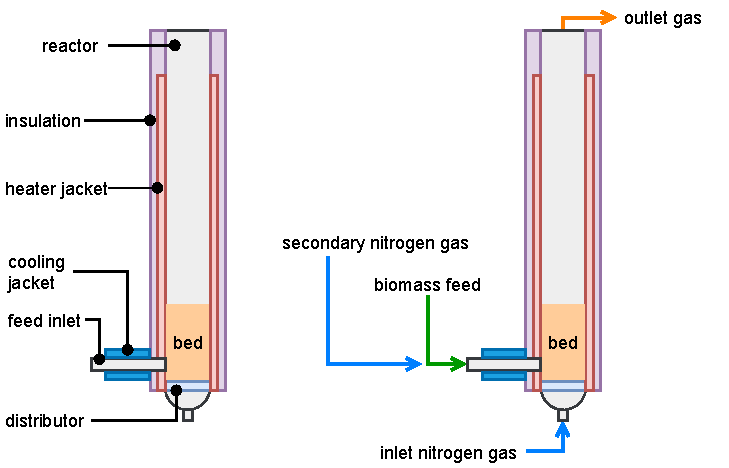
\includegraphics[width=0.8\textwidth]{figures/pyrolyzer1.pdf}
    \caption{Components (left) and inlet/outlet flows (right) of the NREL bubbling fluidized bed pyrolysis reactor.}
    \label{fig:pyrolyzer1}
\end{figure}

Dimensions for the reactor tube, feed inlet, insulation, heat jacket, and distributor plate are given in Figure \ref{fig:pyrolyzer2} and Table \ref{tab:dimensions}. The main reactor tube is a 2-inch Schedule 40 pipe; therefore, the inner and outer reactor diameters are determined from nominal pipe size tables. The gas distributor contains 18 holes in a triangular pattern \cite{French-2019}.

Typical operating conditions of the pyrolyzer are presented in Table \ref{tab:operating}. Pressure drop across the distributor is about 80-90 inches of H$_2$O. Nitrogen gas is used to fluidize the bed and assist biomass particles through the feed inlet tube. Experiments are conducted with an initial mass of sand in the bed; sand is not fed into the reactor during operation. Insulation surrounds the reactor while heat jackets extend almost the entire height of the unit. A cooling jacket surrounds the feed inlet tube. Pyrolysis vapors exit directly out the top of the reactor via a straight tube \cite{French-2019}.

\begin{figure}[H]
    \centering
    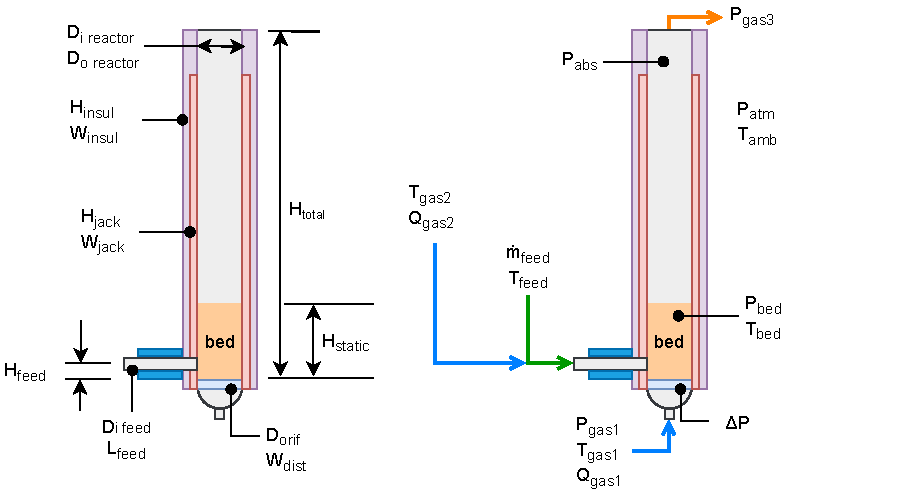
\includegraphics[width=\textwidth]{figures/pyrolyzer2.pdf}
    \caption{Dimensions and typical fast pyrolysis operating conditions for the NREL 2FBR pyrolyzer reactor.}
    \label{fig:pyrolyzer2}
\end{figure}

\begin{table}[H]
    \centering
    \caption{Dimensions for components of the fluidized bed pyrolysis reactor.}
    \label{tab:dimensions}
    \begin{tabular}{llrl}
        \toprule
        Reactor dimension & Symbol & Value & Units \\
        \midrule
        Inner reactor diameter              & D$_{\textrm{i, reactor}}$  & 5.25  & cm \\
        Outer reactor diameter              & D$_{\textrm{o, reactor}}$  & 6.03  & cm \\
        Static bed height                   & H$_{\textrm{static}}$      & 10.16 & cm \\
        Total reactor height                & H$_{\textrm{total}}$       & 43.18 & cm \\
        Feed inlet inner diameter           & D$_{\textrm{i, feed}}$     & 1.27  & cm \\
        Feed height from top of distributor & H$_{\textrm{feed}}$        & 1.9   & cm \\
        Feed inlet tube length              & L$_{\textrm{feed}}$        & 18.29 & cm \\
        Insulation height                   & H$_{\textrm{insul}}$       & 43.18 & cm \\
        Insulation thickness                & W$_{\textrm{insul}}$       & 10    & cm \\
        Jacket height                       & H$_{\textrm{jack}}$        & 35    & cm \\
        Jacket thickness                    & W$_{\textrm{jack}}$        & 5     & cm \\
        Diameter of distributor orifices    & D$_{\textrm{orif}}$        & 0.08  & cm \\
        Thickness of distributor plate      & W$_{\textrm{dist}}$        & 3.17  & mm \\
        Number of orifices in distributor   & n                          & 18    & -- \\
        \bottomrule
    \end{tabular}
\end{table}

\begin{table}[H]
    \centering
    \caption{Typical operating conditions for the fluidized bed pyrolysis reactor. Atmospheric pressure considers elevation of NREL site in Golden, CO.}
    \label{tab:operating}
    \begin{tabular}{llrl}
        \toprule
        Reactor condition & Symbol & Value & Units \\
        \midrule
        Absolute pressure in reactor   & P$_{\textrm{abs}}$  & 101.3     & kPa \\
        Atmospheric pressure           & P$_{\textrm{atm}}$  & 81        & kPa \\
        Ambient air temperature        & T$_{\textrm{amb}}$  & 300.15    & K \\
        Absolute bed pressure          & P$_{\textrm{bed}}$  & 115       & kPa  \\
        Bed temperature                & T$_{\textrm{bed}}$  & 773.15    & K \\
        Pressure drop over distributor & $\Delta$ P          & 21.17     & KPa \\
        Absolute inlet gas pressure    & P$_{\textrm{gas1}}$ & 110--140  & kPa \\
        Inlet gas temperature          & T$_{\textrm{gas1}}$ & 773.15    & K \\
        Inlet gas flowrate             & Q$_{\textrm{gas1}}$ & 14        & SLM (0.29 g/s) \\
        Secondary gas temperature      & T$_{\textrm{gas2}}$ & 298.15    & K \\
        Secondary gas flowrate         & Q$_{\textrm{gas2}}$ & 1.4       & SLM (0.029 g/s) \\
        Absolute outlet gas pressure   & P$_{\textrm{gas3}}$ & 90--110   & kPa \\
        Biomass inlet feedrate         & $\dot{{\textrm{m}}}_{\textrm{feed}}$ & 420 & g/hr \\
        Biomass inlet temperature      & T$_{\textrm{feed}}$ & 298.15    & K \\
        \bottomrule
    \end{tabular}
\end{table}

\subsection{Feedstock proximate and ultimate analyses}

Proximate and ultimate analysis measurements for each feedstock are given in Tables \ref{tab:proximate} and \ref{tab:ultimate} on an as-determined basis (ad). A visual comparison of the proximate and ultimate analysis measurements is shown in Figure \ref{fig:prox-ult-analysis}. Overall, the elemental composition of each feedstock is similar based on the ultimate analysis data. Differences in elemental fractions occur mainly in the C and O fractions with a maximum difference of approximately 3 wt.\% and 5 wt.\% respectively. For the proximate analysis fractions, the largest differences are observed for the fixed carbon (FC) and volatile matter (VM) at 10 wt.\% and 13 wt.\% respectively. A maximum difference of about 3 wt.\% is seen for the ash and moisture fractions.

\begin{table}[H]
    \caption{Proximate analysis measurements given as wt. \% as-determined basis.}
    \label{tab:proximate}
    \centering
    \begin{tabular}{lcrrrrr}
        \toprule
        Name & Cycle & FC & VM & Ash & Moisture & Total \\
        \midrule
        Residues                    & 1  & 20.72 & 72.92 & 1.45 & 4.92 & 100.01 \\
        Stem wood                   & 2  & 16.79 & 79.40 & 0.28 & 3.55 & 100.02 \\
        Bark                        & 3  & 27.16 & 66.29 & 0.70 & 5.86 & 100.01 \\
        Needles                     & 4  & 23.26 & 69.54 & 3.78 & 3.42 & 100.00 \\
        Bark + needles              & 5  & 24.35 & 68.30 & 2.52 & 4.85 & 100.02 \\
        Residues (rep 1)            & 8  & 20.78 & 72.37 & 1.65 & 5.20 & 100.00 \\
        Residues:bark:needles 1:1:1 & 10 & 23.75 & 69.02 & 2.05 & 5.19 & 100.01 \\
        Residues:bark:needles 1:2:2 & 11 & 24.12 & 68.57 & 2.02 & 5.29 & 100.00 \\
        Air classified (10 Hz)      & 12 & 19.92 & 75.59 & 0.92 & 3.57 & 100.00 \\
        Air classified (28 Hz)      & 13 & 18.68 & 76.31 & 0.61 & 4.41 & 100.01 \\
        Whole tree (13 yr)          & 15 & 19.15 & 76.72 & 0.44 & 3.71 & 100.02 \\
        Stem wood (13 yr)           & 16 & 18.60 & 78.37 & 0.30 & 2.75 & 100.02 \\
        \cmidrule{3-6}
        \multicolumn{2}{l}{Maximum difference} & 10.37 & 13.11 & 3.50 & 3.11 & \\
        \bottomrule
    \end{tabular}
\end{table}

\begin{table}[H]
    \caption{Ultimate analysis measurements given as wt. \% as-determined basis.}
    \label{tab:ultimate}
    \centering
    \begin{tabular}{lcrrrrrr}
        \toprule
        Name & Cycle & C & H & O & N & S & Total \\
        \midrule
        Residues                    & 1  & 49.63 & 6.52 & 41.87 & 0.49 & 0.04 & 98.55 \\
        Stem wood                   & 2  & 48.89 & 6.53 & 44.12 & 0.18 & 0.01 & 99.73 \\
        Bark                        & 3  & 51.84 & 6.14 & 40.97 & 0.34 & 0.02 & 99.31 \\
        Needles                     & 4  & 50.22 & 6.22 & 38.77 & 0.92 & 0.09 & 96.22 \\
        Bark + needles              & 5  & 50.35 & 6.18 & 40.21 & 0.67 & 0.06 & 97.47 \\
        Residues (rep 1)            & 8  & 49.82 & 6.56 & 41.34 & 0.58 & 0.05 & 98.35 \\
        Residues:bark:needles 1:1:1 & 10 & 50.58 & 6.31 & 40.43 & 0.59 & 0.05 & 97.96 \\
        Residues:bark:needles 1:2:2 & 11 & 50.86 & 6.24 & 40.24 & 0.58 & 0.06 & 97.98 \\
        Air classified (10 Hz)      & 12 & 50.16 & 6.46 & 42.06 & 0.37 & 0.03 & 99.08 \\
        Air classified (28 Hz)      & 13 & 48.93 & 6.42 & 43.77 & 0.26 & 0.02 & 99.40 \\
        Whole tree (13 yr)          & 15 & 49.32 & 6.44 & 43.48 & 0.30 & 0.02 & 99.56 \\
        Stem wood (13 yr)           & 16 & 49.40 & 6.41 & 43.68 & 0.21 & 0.01 & 99.71 \\
        \cmidrule{3-7}
        \multicolumn{2}{l}{Maximum difference} & 2.95 & 0.42 & 5.35 & 0.74 & 0.08 & \\
        \bottomrule
    \end{tabular}
\end{table}

\begin{figure}[H]
    \centering
    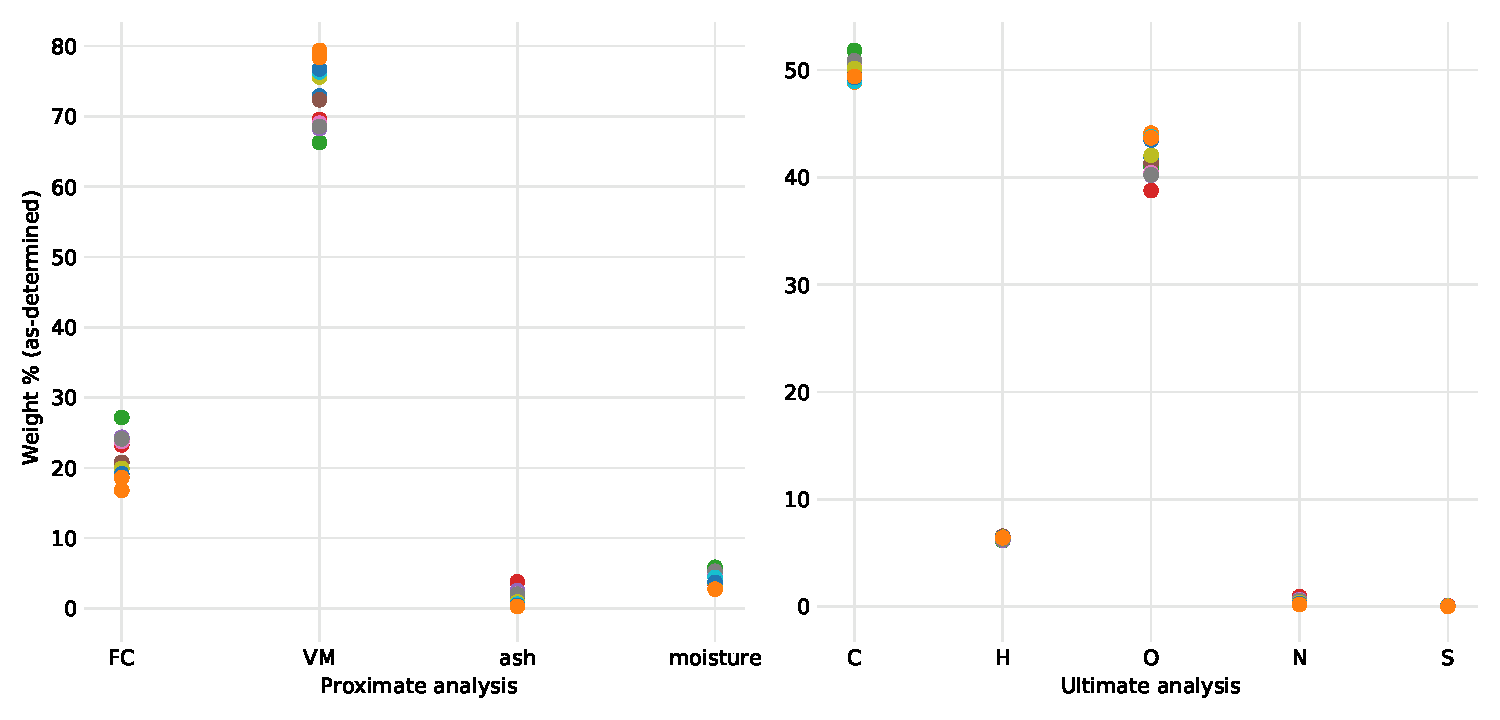
\includegraphics[width=\textwidth]{figures/prox-ult-analysis.pdf}
    \caption{Comparison of proximate (left) and ultimate (right) analysis measurements for each feedstock. Values represent wt. \% as-determined basis.}
    \label{fig:prox-ult-analysis}
\end{figure}

\subsection{Feedstock chemical analysis}

Chemical analysis data for each feedstock was supplied by the Idaho National Laboratory on a wt. \% dry basis (D). A summary of the chemical analysis measurements is given in Tables \ref{tab:chemical-1} and \ref{tab:chemical-2}. A comparison of the values are shown in Figure \ref{fig:chem-analysis}. The largest variations in the measured chemical fractions occur for the lignin and glucan with a maximum difference of 15 wt. \% and 17.5 wt. \% respectively.

\begin{table}[H]
    \caption{Chemical analysis measurements given as weight percent (wt. \%) dry basis (D).}
    \label{tab:chemical-1}
    \centering
    \begin{tabular}{lrrrrrr}
        \toprule
        Chemical component & \rotatebox{90}{Residues} & \rotatebox{90}{Stem wood} & \rotatebox{90}{Bark} & \rotatebox{90}{Needles} & \rotatebox{90}{Bark + needles} & \rotatebox{90}{Residues (rep 1)} \\
        \midrule
        structural inorganics      & 0.94  & 0.32   & 0.5    & 3.23  & 1.76  & 1.24  \\
        non-structural inorgranics & 0.37  & 0      & 0.08   & 0.56  & 0.66  & 0.19  \\
        water extractives          & 4.91  & 2.76   & 2.9    & 5.95  & 4.01  & 6.18  \\
        ethanol extractives        & 0.62  & 0.31   & 0.46   & 1.35  & 0.98  & 0.68  \\
        acetone extractives        & 6.6   & 2.57   & 3.33   & 7.35  & 5.53  & 7.88  \\
        lignin                     & 35.52 & 30.7   & 34.34  & 41.03 & 45.88 & 35.22 \\
        glucan                     & 28.18 & 39.84  & 33.83  & 22.33 & 22.75 & 26.48 \\
        xylan                      & 7.33  & 6.3    & 7.74   & 4.12  & 4.17  & 6.52  \\
        galactan                   & 3.56  & 2.59   & 3.68   & 2.57  & 3.28  & 3.44  \\
        arabinan                   & 1.93  & 0      & 3.5    & 1.52  & 2.4   & 2.84  \\
        mannan                     & 7.64  & 14.94  & 9.15   & 7.44  & 5.35  & 6.33  \\
        acetyl                     & 0.95  & 1.35   & 1.21   & 0.98  & 0.81  & 0.94  \\
        \cmidrule{2-7}
        total                      & 98.55 & 101.68 & 100.72 & 98.43 & 97.58 & 97.94 \\
        \bottomrule
    \end{tabular}
\end{table}

\begin{table}[H]
    \caption{Chemical analysis measurements given as weight percent (wt. \%) dry basis (D).}
    \label{tab:chemical-2}
    \centering
    \begin{tabular}{lrrrrrr}
        \toprule
        Chemical component & \rotatebox{90}{Residues:bark:needles 1:1:1} & \rotatebox{90}{Residues:bark:needles 1:2:2} & \rotatebox{90}{Air classified (10 Hz)} & \rotatebox{90}{Air classified (28 Hz)} & \rotatebox{90}{Whole tree (13 yr)} & \rotatebox{90}{Stem wood (13 yr)} \\
        \midrule
        structural inorganics      & 1.66  & 1.91  & 0.55  & 0.38   & 0.5   & 0.32   \\
        non-structural inorgranics & 0.02  & 0.21  & 0.31  & 0.22   & 0.08  & 0      \\
        water extractives          & 5.76  & 5.53  & 3.26  & 1.76   & 2.9   & 1.56   \\
        ethanol extractives        & 1.02  & 1.04  & 0.44  & 0.31   & 0.46  & 0.34   \\
        acetone extractives        & 6.87  & 6.51  & 4.02  & 2.4    & 3.33  & 1.76   \\
        lignin                     & 42.06 & 42.9  & 35.11 & 35.23  & 33.34 & 33.4   \\
        glucan                     & 23.37 & 22.92 & 31.99 & 34.37  & 33.83 & 38.15  \\
        xylan                      & 5.07  & 4.64  & 7.63  & 8.39   & 7.74  & 7.97   \\
        galactan                   & 2.95  & 3.03  & 3.63  & 3.9    & 3.68  & 3.63   \\
        arabinan                   & 1.62  & 2.23  & 1.34  & 0      & 3.5   & 3.53   \\
        mannan                     & 7.55  & 5.91  & 10.01 & 12.41  & 9.15  & 10.08  \\
        acetyl                     & 0.9   & 0.85  & 1.18  & 1.24   & 1.21  & 1.41   \\
        \cmidrule{2-7}
        total                      & 98.85 & 97.68 & 99.47 & 100.61 & 99.72 & 102.15 \\
        \bottomrule
    \end{tabular}
\end{table}

\begin{figure}[H]
    \centering
    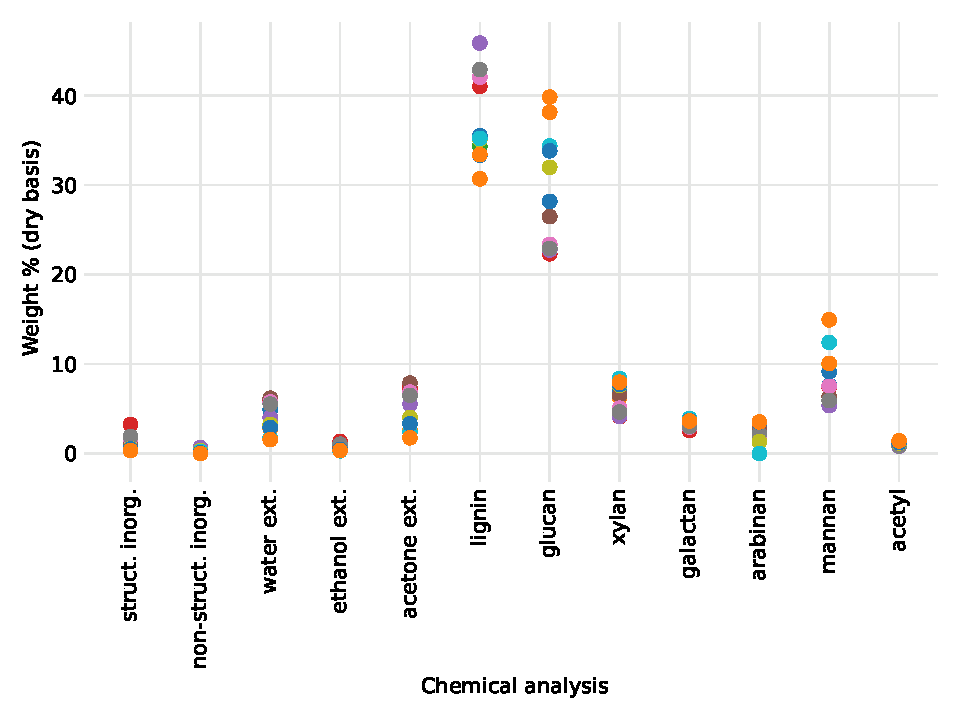
\includegraphics[width=0.8\textwidth]{figures/chem-analysis.pdf}
    \caption{Comparison of chemical analysis measurements for each feedstock.}
    \label{fig:chem-analysis}
\end{figure}

\subsection{Bed particle characteristics}

Characteristics of the sand particles that represent the fluidized bed material were obtained by NETL and are summarized in Table \ref{tab:sand}. A microscope image of the sand particles is shown in Figure \ref{fig:sand}. The particle density was determined from a helium pycnometer while size distribution and sphericity was obtained from QICPIC image analysis \cite{Netl-2021}. At the time of writing this report, bed particle characteristics were not utilized in the reactor models discussed in subsequent sections.

\begin{table}[H]
    \caption{Bed material (sand) characteristics.}
    \label{tab:sand}
    \centering
    \begin{tabular}{lcrl}
        \toprule
        Parameter & Symbol & Value & Units \\
        \midrule
        Particle envelope density     & $\rho$ & 2.7051 & g/cm$^3$ \\
        Standard deviation of density & --     & 0.0004 & g/cm$^3$ \\
        Sauter mean diameter          & SMD    & 509    & $\mu$m \\
        Average particle sphericity   & $\phi$ & 0.874  & -- \\
        \bottomrule
    \end{tabular}
\end{table}

\begin{figure}[H]
    \centering
    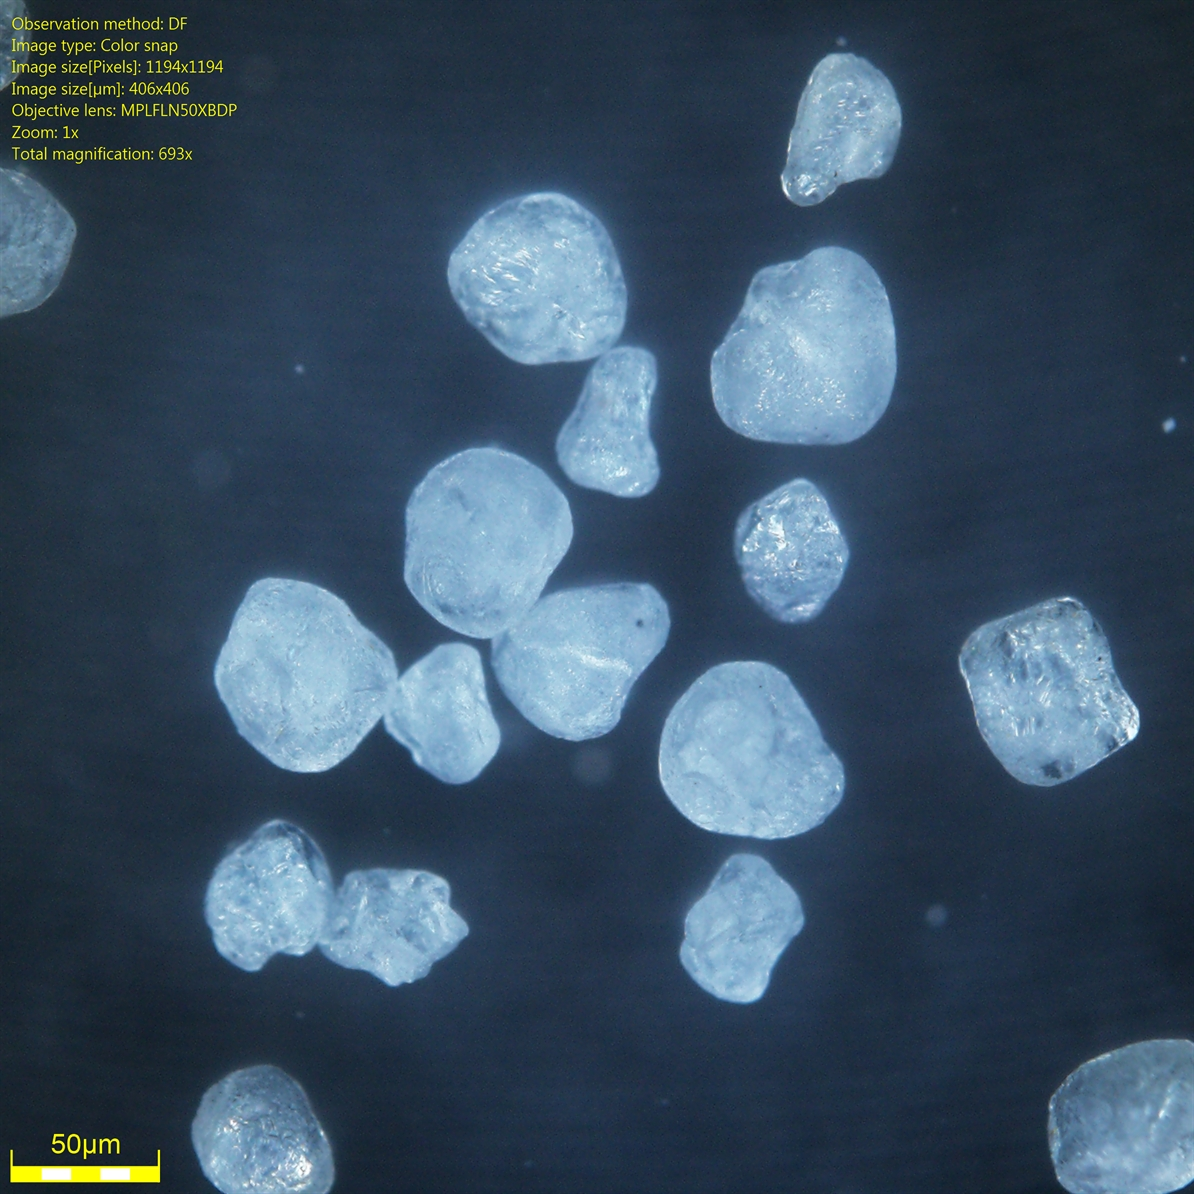
\includegraphics[width=0.5\textwidth]{figures/sand.jpg}
    \caption{Microscope image of sand particles used for the bed material.}
    \label{fig:sand}
\end{figure}

\subsection{Product yields}

Product yields measured from the fast pyrolysis of each feedstock in the fluidized bed reactor are given in Table \ref{tab:yields}. A comparison of the product yields from each feedstock is shown in Figure \ref{fig:yields}. The oil and char yields are the most variable between the different feedstocks while condensables and water vapor differ by a few percent.

\begin{table}[H]
    \caption{Measured reactor yields from each feedstock experiment. Values expressed as percent wet basis (w).}
    \label{tab:yields}
    \centering
    \begin{tabular}{lcccccr}
        Feedstock & \rotatebox{90}{Oil} & \rotatebox{90}{Condensables} & \rotatebox{90}{Light gas} & \rotatebox{90}{Water vapor} & \rotatebox{90}{Char} & \rotatebox{90}{Total} \\
        \toprule
        Residues                    & 63.5 & 1.6 & 14.7 & 0.4 & 15.2 & 95.4 \\
        Stem wood                   & 72.3 & 2.8 & 14.1 & 1.2 & 10.9 & 101.3 \\
        Bark                        & 58.3 & 1.3 & 11.4 & 0.8 & 31.9 & 103.7 \\
        Needles                     & 55.4 & 2.7 & 14.5 & 0.6 & 25.6 & 98.8 \\
        Bark + needles              & 55.5 & 1.3 & 15.1 & 1.2 & 16.5 & 89.6 \\
        Residues (rep 1)            & 62.6 & 2.5 & 15.9 & 2.5 & 17.3 & 100.8 \\
        Residues:bark:needles 1:1:1 & 58.3 & 3.1 & 14.3 & 0.7 & 24.6 & 101.0 \\
        Residues:bark:needles 1:2:2 & 57.1 & 0.6 & 15.0 & 2.0 & 25.0 & 99.7 \\
        Air classified (10 Hz)      & 57.6 & 3.0 & 16.2 & 3.2 & 16.3 & 96.3 \\
        Air classified (28 Hz)      & 65.0 & 2.5 & 17.9 & 1.6 & 13.9 & 100.9 \\
        Whole tree (13 yr)          & 63.1 & 1.8 & 17.7 & 2.1 & 13.9 & 98.6 \\
        Stem wood (13 yr)           & 67.8 & 1.9 & 15.2 & 3.2 & 12.2 & 100.3 \\
        \bottomrule
    \end{tabular}
\end{table}

\begin{figure}[H]
    \centering
    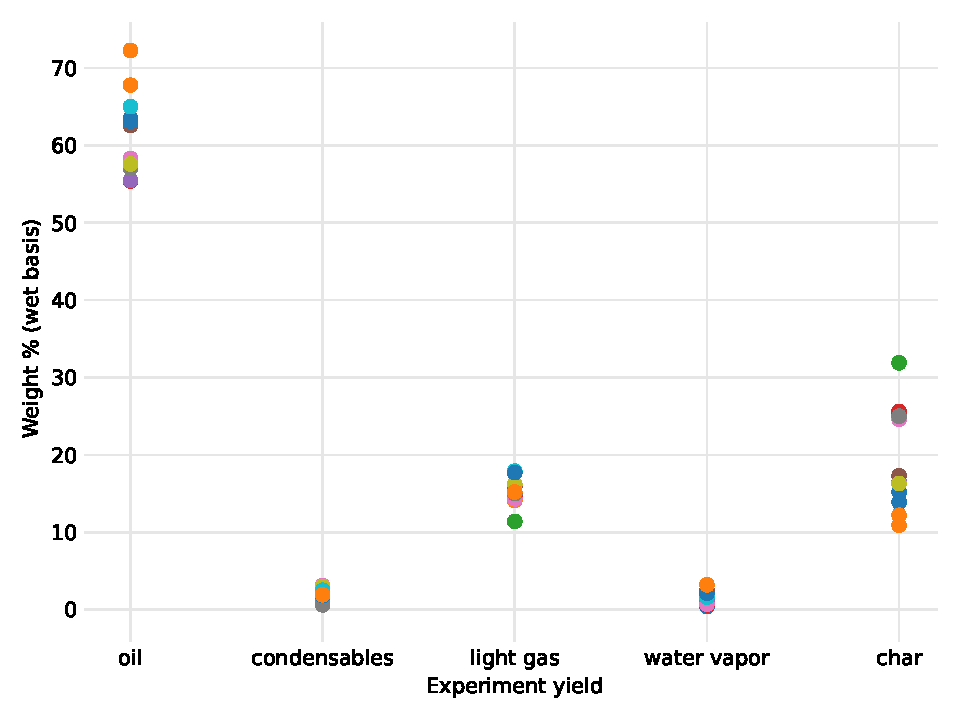
\includegraphics[width=0.8\textwidth]{figures/yields.pdf}
    \caption{Comparison of the measured product yields for each feedstock. Values shown as percent wet basis.}
    \label{fig:yields}
\end{figure}
